\chapter{原子光谱}

\begin{introduction}
	\item 原子发射光谱的分析方法
	\item 原子发射光谱的仪器
	\item 原子吸收光谱分析
\end{introduction}


%设计方案:
%1.定义、概念、原理,做个环境
%2.公式、符号说明环境
%3.步骤、结构、小点:列表
%4.对比:表格

\section{原子发射光谱的分析方法}
%1、原子发射光谱定性分析:不同元素的原子能级结构不同,因此能级跃迁所产生的谱线具有不同的波长特征。根据谱线特征可以进行发射光谱定性分析。什么是共振线?什么是自吸收?原子发射光谱定量分析:罗马金-赛伯公式

不同元素的原子能级结构不同,因此能级跃迁所产生的谱线具有不同的波长特征。每一种元素的原子都有其特征光谱。
\subsection{定性分析}

\begin{definition*}{共振线(特征谱线)}{}
	元素由基态到第一激发态的跃迁对应的谱线称为共振线。
	\begin{itemize}
		\item 这种跃迁最容易发生,需要的能量最低,产生的谱线也最强。
	\end{itemize}
\end{definition*}

\begin{definition*}{灵敏线}{}
	元素特征谱线中强度较大的称为元素的灵敏线。

\begin{itemize}
	\item 如果在光谱中检出了某元素的灵敏线,可以确证试样中存在该元素,但是至少要有两条灵敏线出现,才可以确认该元素的存在。
	\item 如果未检出灵敏线,说明试样中不存在备件元素或元素含量在灵敏度以下。
\end{itemize}
\end{definition*}

\subsection{定量分析}

\begin{theorem*}{罗马金-赛伯公式}{}
	\begin{gather*}
		I=A\cdot c^b\\
		\lg I = b \lg c + \lg A
	\end{gather*}
	
	$I$是两个能级之间的谱线强度;$A$代表两个能级间每个原子单位时间内发生$A$次跃迁(即跃迁几率);$c$是样品中分析物的浓度;$b$是自吸系数,随浓度$c$增加而减小,当浓度很小而无自吸时,$b=1$。
\end{theorem*}


一般采用内标法、标准加入法进行分析。

\begin{definition*}{自吸收}{}
	光源等离子体中心部位原子发射的光子通过温度较低的外层时,被外层基态原子吸收的现象。
\end{definition*}

\section{原子发射光谱的仪器}
%2、原子发射光谱仪的光源作用?有哪些类型?

原子发射光谱的光源称为激发光源。
\begin{itemize}
	\item 作用:\textbf{提供试样中被测元素蒸发、原子化和原子激发发光所需要的的能量}。
	\item 要求:灵敏度高、重现性好、光谱背景小,结构简单、操作安全。
	\item 类型:火焰光源、电弧光源、高压电容火花光源、辉光放电光源、电感耦合高频等离子体光源(ICP光源)
\end{itemize}

\subsection{直流电弧光源}
\begin{itemize}
	\item 电机温度高,弧焰中心温度为$5000\sim 7000\mathrm{K}$,有利于试样的蒸发;
	\item 除石墨电极产生的氰带光谱外,背景比较浅;
	\item 电弧在电极表面无常游动,且有分馏效应\footnote{不同物质因沸点不同而导致蒸发速度不同},重现性比较差;
	\item 谱线容易发生自吸收现象。
	\item 常用于定性分析以及矿石、矿物难熔物质中痕量组分的定量测定。
\end{itemize}

\begin{figure}[!h]
	\centering
	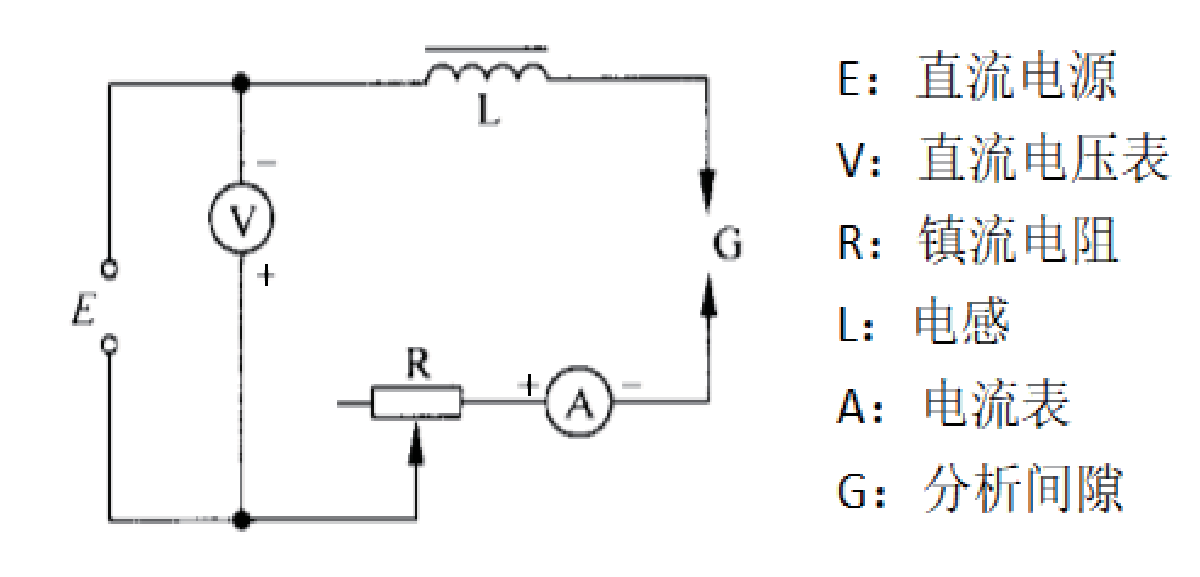
\includegraphics[width=0.6\linewidth]{image/chp8_circuit_diagram1.eps}
%	\caption{}
	\label{fig:chp8circuitdiagram1}
\end{figure}


\subsection{低压交流电弧光源}

\begin{itemize}
	\item 电极温度较直流电弧略低;
	\item 因电弧弧温较高,灵敏度比直流电弧高;
	\item 弧焰稳定,适于定量分析。
\end{itemize}

\begin{figure}[!h]
	\centering
	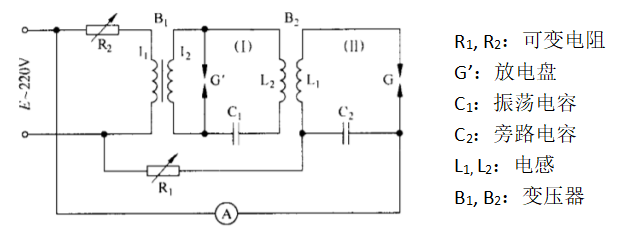
\includegraphics[width=0.7\linewidth]{image/chp8_circuit_diagram2}
%	\caption{}
	\label{fig:chp8circuitdiagram2}
\end{figure}

\subsection{高压电容火花光源}
\begin{itemize}
	\item 火花作用于电极的面积小,时间短,电极温度低,不适于难蒸发的物质;
	\item 火花放电的能量高,能激发电位很高的原子线或离子线;
	\item 稳定性好,适于定量分析;
	\item 电极面积小,适于微区分析。
\end{itemize}

\begin{figure}[!h]
	\centering
	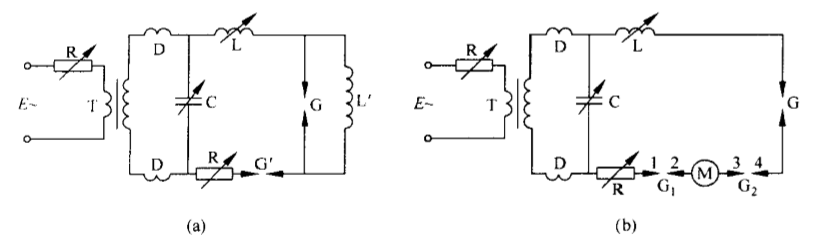
\includegraphics[width=0.7\linewidth]{image/chp8_circuit_diagram3}
	\caption{(a)稳定间隙控制的火花电路;(b)旋转间隙控制的火花电路\\
		E:电源;R:可变电阻;T:升压变压器;D:扼流圈;C:可变电容;L:可变电感;L’:高阻抗自感线圈;G:分析间隙;G’:控制间隙;G1,G2:断续控制间隙;M:同步电机带动的断续器}
	\label{fig:chp8circuitdiagram3}
\end{figure}

电弧和火花光源适用于固体样品分析,但温度低,基体影响严重,需要寻找更高蒸发、原子化和激发的光源。

\begin{note}
	基体效应:指试样组成对谱线强度的影响,主要发生在试样的蒸发和激发过程中。试样中占大多数的物质的沸点高低决定蒸发温度的高低;主体成分的电离电位越高,光源激发温度越高,影响谱线强度。不同蒸发顺序也影响谱线强度。
\end{note}

\subsection{辉光放电光源}
Grimm辉光放电管用于固体样品表面分析,能检测$\ce{B,C,Si,P,S}$等元素。

\begin{figure}[!h]
	\centering
	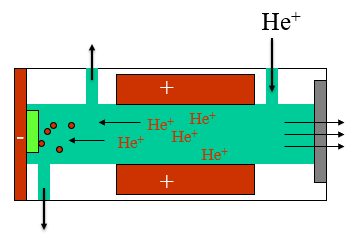
\includegraphics[width=0.6\linewidth]{image/chp8_huiguang}
%	\caption{}
	\label{fig:chp8huiguang}
\end{figure}


\subsection{ICP光源(inductively coupled plasma)}
\begin{itemize}
	\item 组成:高频发生器和感应圈、等离子炬管和供气系统、试样引入系统;
	\item 优势:
	\begin{itemize}
		\item 具有趋肤效应\footnote{涡流主要集中在等离子体的表面层,气溶胶从中心通道进入},自吸效应小;
		\item 温度高,基底成分被分解,减小基底效应;
		\item 不需要电极,无电极污染、加热方式具有良好稳定性;
		\item 电子密度高,电离干扰可不考虑。
	\end{itemize}
	\item 缺点:固体进样较困难,对气体和非金属灵敏度低;雾化效率低;设备和维持费高。
\end{itemize}

\begin{figure}[!h]
	\centering
	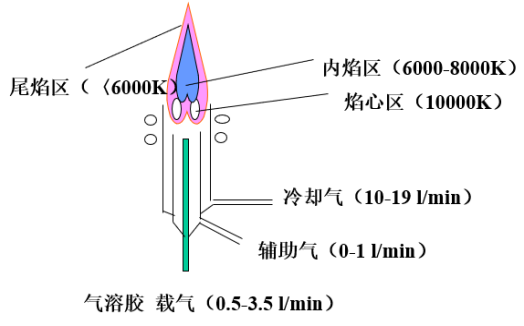
\includegraphics[width=0.7\linewidth]{image/chp8_ICP}
%	\caption{}
	\label{fig:chp8icp}
\end{figure}

\begin{itemize}
	\item 外管:通冷却气$\ce{Ar}$使等离子体离开外层石英管内壁,避免它烧毁石英管。
	\item 中层石英管:出口做成喇叭形,通入$\ce{Ar}$气维持等离子体作用。
	\item 内层石英管:把载气载带试样气溶胶(由气动或超声雾化器产生)注入等离子体内。
	\item 内焰区:(测光区)分析物原子化、激发、电离与辐射的主要区域。
	\item 焰心区:(预热区)等离子体与高频感应线圈耦合获得能量的区域;试样气溶胶被预热、挥发溶剂、蒸发溶质。
	\item 尾焰区:温度低,只能激发低能级的谱线。
\end{itemize}


\section{原子吸收光谱}
%3、原子吸收光谱定量分析?原子吸收光谱仪的结构组成?光源——空心阴极灯。

\subsection{原子吸收光谱定量分析}
原子吸收光谱产生于基态原子对特征谱线的吸收。

实验条件一定时,基本关系式可以简写为$A=kc$,即吸光度和(质量体积)浓度成正比。

原子吸收光谱轮廓图如图\ref{fig:chp8absorption},以原子吸收谱线的中心波长和半宽度来表征。
\textit{中心波长}由原子能级决定;\textit{半宽度}指在中心波长附近,极大吸收系数一半处,吸收光谱线轮廓上两点之间的频率差或波长差。

\begin{figure}[!h]
	\centering
	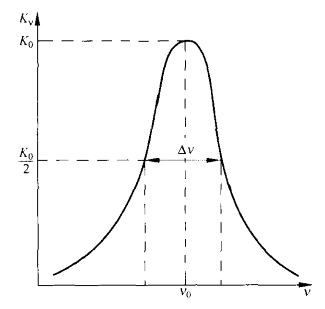
\includegraphics[width=0.5\linewidth]{image/chp8_absorption}
	\caption{}
	\label{fig:chp8absorption}
\end{figure}

原子光谱分析的优点是:
\begin{itemize}
	\item 检出限低,灵敏度高。检出限最低可达$10^{-10}\sim 10^{-14}\mathrm{g}$;
	\item 测量精度好;
	\item 分析速度快;
	\item 应用范围广,可测定金属元素,也可通过间接原子吸收法测非金属和有机化合物等;
	\item 仪器简单,操作方便;
\end{itemize}

\subsection{原子吸收光谱仪的结构}

\begin{figure}[!h]
	\centering
	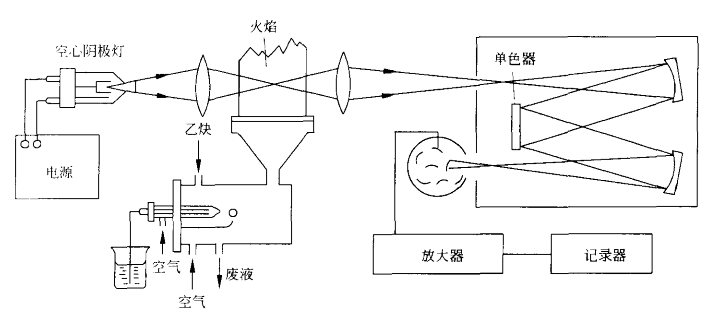
\includegraphics[width=0.7\linewidth]{image/chp8_instrument}
%	\caption{}
	\label{fig:chp8instrument}
\end{figure}

\subsubsection{光源}
空心阴极灯是最理想、应用最广的光源,用来发射被测元素的特征共振辐射。它满足对光源的各项基本要求:
\begin{itemize}
	\item 发射的共振辐射的半宽度要明显小于吸收线的半宽度;
	\item 辐射强度大;
	\item 背景低,低于特征共辐射强度的1\%;
	\item 稳定性好;
	\item 使用寿命长于5A·h
\end{itemize}

工作原理:
\begin{itemize}
	\item 由一个由被测元素材料制成的空心阴极和一个由钛、锆、钽或其他材料制作的阳极。
	\item 玻璃管内由260~1300Pa的惰性气体氖或氩来载带电流,使阴极产生溅射及激发原子发射特征的锐线光谱。
	\item 云母屏蔽片来使放电限制在阴极腔内,同时使阴极定位。
	\item 采用低压辉光放电,集中于阴极空腔内。
	\item 光源调制:使用脉冲供电方式来改善放电特性,同时便于使有用的原子吸收信号与原子化器的滞留发射信号区分开。
\end{itemize}

\begin{figure}[!h]
	\centering
	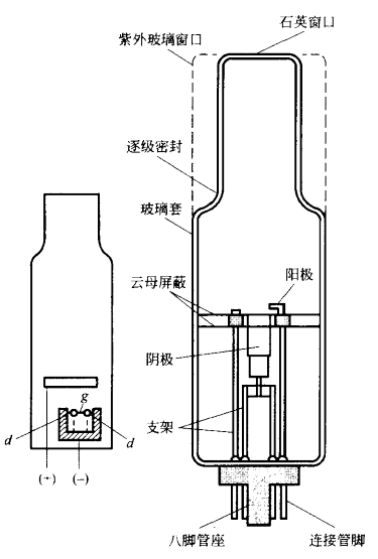
\includegraphics[width=0.4\linewidth]{image/chp8_ICP_lamp}
	\caption{}
	\label{fig:chp8icplamp}
\end{figure}

\subsubsection{原子化器}
作用:提供能量,使试样干燥、蒸发和原子化。

有三种原子化的方法:

\begin{itemize}
	\item 火焰原子化法
	\begin{itemize}
		\item 采用最多的是乙炔-空气火焰,其燃烧稳定,重现性好,噪声低,燃烧速度不太高,温度足够高,对大多数元素有足够灵敏度。
		\item 氢-空气火焰是氧化性火焰,燃烧速度高于乙炔-空气,优点是背景较弱,透射性好,但温度较低。
		\item 乙炔-氧化亚氮高温火焰温度在三者中最高,燃烧速度不快,可测定70多种元素。
	\end{itemize}
	\item 非火焰原子化法
	常用管式石墨炉。
	\begin{itemize}
		\item 优点是试样原子化在惰性气体和强还原性介质进行,利于氧化物分解和自由原子生成;用样量小,样品利用率高,绝对灵敏度高;固、液试样均可直接进样。
		\item 缺点是试样组成不均匀性影响较大,背景吸收强,精密度不如火焰原子化法。
	\end{itemize}
	\item 低温原子化法
		利于某些元素(如$\ce{Hg}$)单质或其氢化物(如$\ce{AsH3}$)在低温下的易挥发性,将其导入气体流动吸收池反应出单质或氢化物后,进行原子化。目前通过该方法测定$\ce{Hg, As, Sb, Se, Sn, Bi, Ge, Pb, Te}$等。
\end{itemize}

\subsubsection{分光器}
将所需要的共振吸收线分离出来,由入射和出射狭缝、反射镜和色散元件(光栅)组成。

\subsubsection{检测系统}
\begin{itemize}
	\item 光电倍增管
光电倍增管的外壳由玻璃或石英制成,内部抽真空,阴极涂有能发射电子的光敏物质,如$\ce{Sb-Cs}$或$\ce{Ag-O-Cs}$等,在阴极C和阳极A间装有一系列次级电子发射极,即电子倍增极D1、D2 … 等。阴极C和阳极A之间加有约1000V的直流电压,当辐射光子撞击光阴极C时发射光电子,该光电子被电场加速落在第一被增极D1上,撞击出更多的二次电子,依次类推,阳极最后收集到的电子数将是阴极发出的电子数的$10^5\sim 10^8$倍。
	\item CCD
电荷耦合器件,优点是速度快、动态响应范围和灵敏度均可能达到或超过光电倍增管,且性能稳定、体积小、耐用。
\end{itemize}

